\documentclass[tikz,border=5pt]{standalone}
\usepackage{tikz}
\usetikzlibrary{arrows.meta,positioning,calc,fit,shapes.geometric,decorations.pathreplacing}
\usepackage{amsmath,amssymb}

\definecolor{ink}{RGB}{45,52,58}
\definecolor{grayA}{RGB}{118,126,134}
\definecolor{blueA}{RGB}{55,110,180}
\definecolor{greenA}{RGB}{72,140,88}
\definecolor{purpleA}{RGB}{137,90,162}
\definecolor{orangeA}{RGB}{204,116,52}
\definecolor{tealA}{RGB}{53,132,138}

\begin{document}
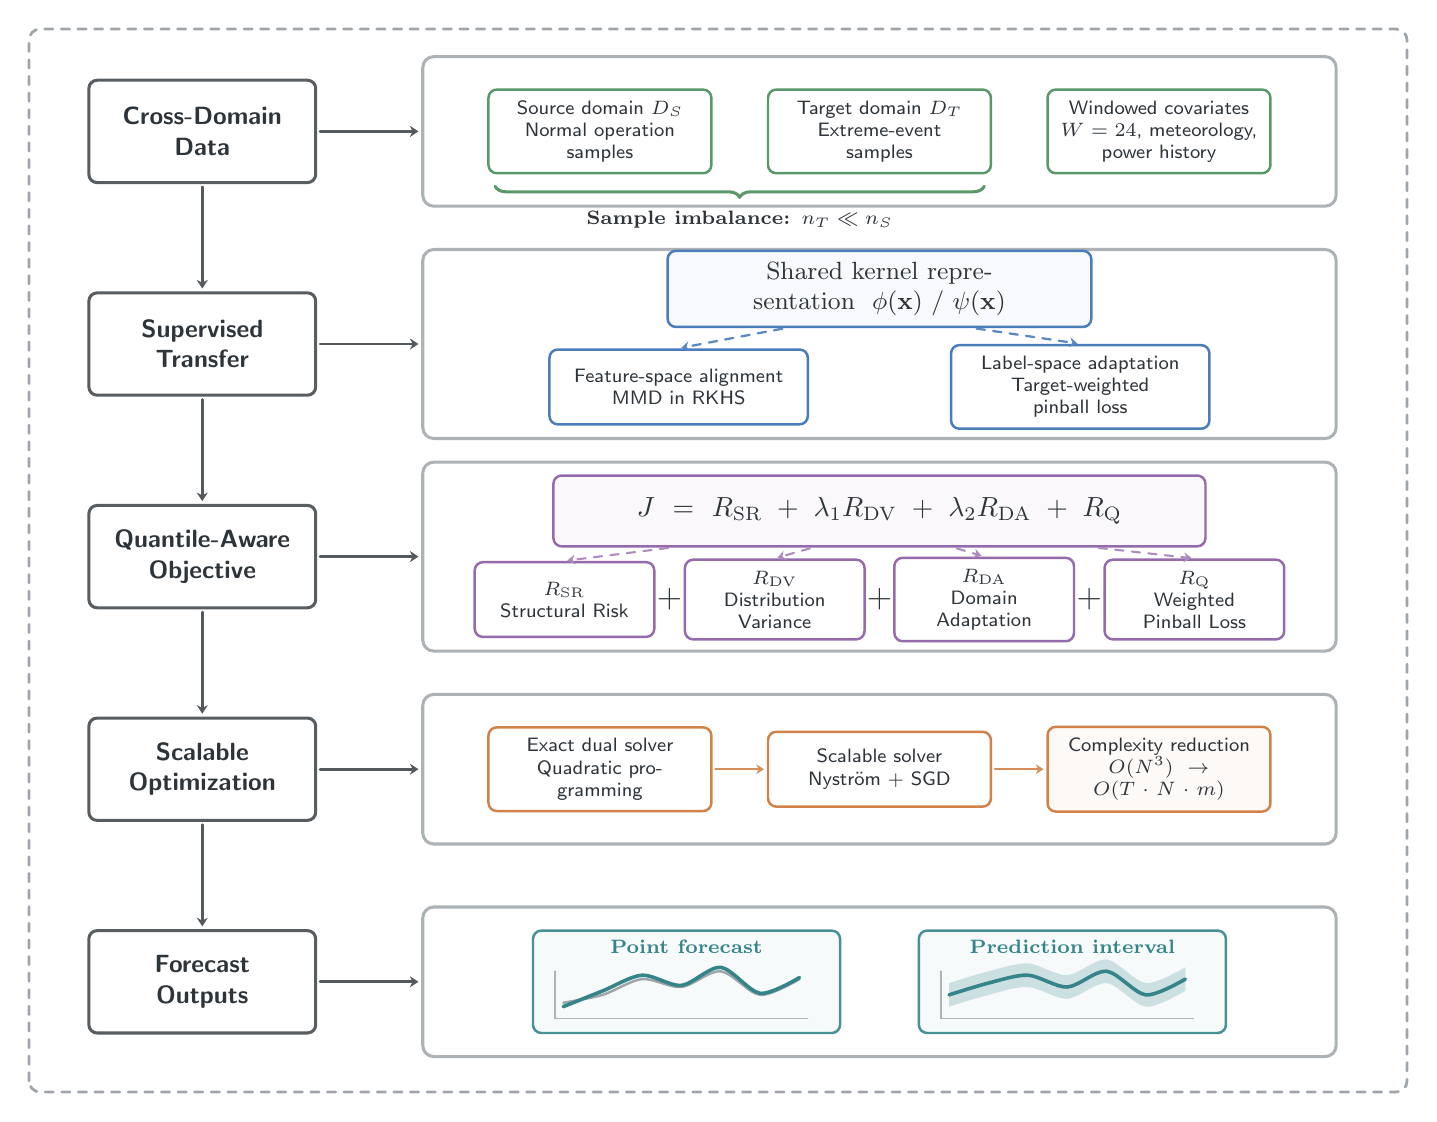
\begin{tikzpicture}[
  line cap=round,
  line join=round,
  font=\small\sffamily,
  leftbox/.style={
    draw=ink!80, fill=white, rounded corners=3pt,
    line width=1.1pt, align=center, text width=2.6cm,
    minimum height=1.3cm, inner sep=4pt, font=\small\bfseries\sffamily, text=ink
  },
  panel/.style={
    draw=grayA!60, fill=white, rounded corners=4pt,
    line width=1.1pt, minimum width=11.6cm, inner sep=0pt
  },
  cbox/.style={
    draw=#1!90, fill=white, rounded corners=3pt,
    line width=0.9pt, align=center, inner sep=4pt, font=\scriptsize\sffamily, text=ink
  },
  cboxfill/.style={
    draw=#1!90, fill=#1!4, rounded corners=3pt,
    line width=0.9pt, align=center, inner sep=4pt, font=\scriptsize\sffamily, text=ink
  },
  flow/.style={
    draw=ink!82, line width=0.95pt, shorten >=1pt, shorten <=1pt,
    -{Stealth[length=3.1pt,width=4.0pt]}
  },
  soft/.style={
    draw=#1!82, line width=0.82pt, shorten >=1pt, shorten <=1pt,
    -{Stealth[length=2.8pt,width=3.5pt]}
  },
  note/.style={font=\scriptsize, text=grayA!95}
]

% Geometry
\coordinate (lx) at (2.0,0);
\coordinate (rx) at (10.6,0);

\def\hspacing{2.7}
\coordinate (r1) at (0, 10.8);
\coordinate (r2) at (0, 8.1);
\coordinate (r3) at (0, 5.4);
\coordinate (r4) at (0, 2.7);
\coordinate (r5) at (0, 0.0);

% Outer frame
\draw[draw=grayA!70, dashed, line width=1pt, rounded corners=4pt] (-0.2,-1.4) rectangle (17.3, 12.1);

% ------------------------------------------------------------------
% Left pipeline
\node[leftbox] (s1) at ($(lx)+(r1)$) {Cross-Domain\\Data};
\node[leftbox] (s2) at ($(lx)+(r2)$) {Supervised\\Transfer};
\node[leftbox] (s3) at ($(lx)+(r3)$) {Quantile-Aware\\Objective};
\node[leftbox] (s4) at ($(lx)+(r4)$) {Scalable\\Optimization};
\node[leftbox] (s5) at ($(lx)+(r5)$) {Forecast\\Outputs};

\draw[flow] (s1.south) -- (s2.north);
\draw[flow] (s2.south) -- (s3.north);
\draw[flow] (s3.south) -- (s4.north);
\draw[flow] (s4.south) -- (s5.north);

% ------------------------------------------------------------------
% Right panels
\node[panel, minimum height=1.9cm] (p1) at ($(rx)+(r1)$) {};
\node[panel, minimum height=2.4cm] (p2) at ($(rx)+(r2)$) {};
\node[panel, minimum height=2.4cm] (p3) at ($(rx)+(r3)$) {};
\node[panel, minimum height=1.9cm] (p4) at ($(rx)+(r4)$) {};
\node[panel, minimum height=1.9cm] (p5) at ($(rx)+(r5)$) {};

\draw[flow] (s1.east) -- (p1.west);
\draw[flow] (s2.east) -- (p2.west);
\draw[flow] (s3.east) -- (p3.west);
\draw[flow] (s4.east) -- (p4.west);
\draw[flow] (s5.east) -- (p5.west);

% ------------------------------------------------------------------
% Panel 1: inputs
\node[cbox=greenA, text width=2.55cm, minimum height=0.95cm] (p11) at ($(p1.center)+(-3.55,0)$)
{Source domain $D_S$\\Normal operation\\samples};
\node[cbox=greenA, text width=2.55cm, minimum height=0.95cm] (p12) at ($(p1.center)+(0,0)$)
{Target domain $D_T$\\Extreme-event\\samples};
\node[cbox=greenA, text width=2.55cm, minimum height=0.95cm] (p13) at ($(p1.center)+(3.55,0)$)
{Windowed covariates\\$W=24$, meteorology,\\power history};

\draw[decorate,decoration={brace,amplitude=4pt,mirror}, draw=greenA!90, line width=1.1pt] 
  ($(p11.south west)+(0.1,-0.15)$) -- ($(p12.south east)+(-0.1,-0.15)$) 
  node[midway, below=5pt, font=\scriptsize\bfseries, text=ink] {Sample imbalance: $n_T \ll n_S$};

% ------------------------------------------------------------------
% Panel 2: transfer
\node[cboxfill=blueA, text width=5.1cm, minimum height=0.9cm, font=\small] (p21) at ($(p2.center)+(0,0.70)$)
{Shared kernel representation \ $\phi(\mathbf{x})$ / $\psi(\mathbf{x})$};

\node[cbox=blueA, text width=3.00cm, minimum height=0.95cm] (p22) at ($(p2.center)+(-2.55,-0.545)$)
{Feature-space alignment\\MMD in RKHS};
\node[cbox=blueA, text width=3.00cm, minimum height=0.95cm] (p24) at ($(p2.center)+(2.55,-0.545)$)
{Label-space adaptation\\Target-weighted pinball loss};

% Dashed arrow: shared kernel -> feature-space alignment (left)
\draw[draw=blueA!82, dashed, line width=0.82pt, shorten >=1pt, shorten <=1pt, -{Stealth[length=2.8pt,width=3.5pt]}]
  (p21.south) ++(-1.2,0) -- (p22.north);
% Dashed arrow: shared kernel -> label-space adaptation (right)
\draw[draw=blueA!82, dashed, line width=0.82pt, shorten >=1pt, shorten <=1pt, -{Stealth[length=2.8pt,width=3.5pt]}]
  (p21.south) ++(1.2,0) -- (p24.north);

% ------------------------------------------------------------------
% Panel 3: objective
\node[cboxfill=purpleA, text width=8.0cm, minimum height=0.9cm, font=\normalsize] (p31) at ($(p3.center)+(0,0.58)$)
{$J = R_{\mathrm{SR}} \,+\, \lambda_1 R_{\mathrm{DV}} \,+\, \lambda_2 R_{\mathrm{DA}} \,+\, R_{\mathrm{Q}}$};

\node[cbox=purpleA, text width=2.0cm, minimum height=0.95cm] (p32) at ($(p3.center)+(-4.0,-0.545)$)
{$R_{\mathrm{SR}}$\\Structural Risk};
\node[cbox=purpleA, text width=2.0cm, minimum height=0.95cm] (p33) at ($(p3.center)+(-1.33,-0.545)$)
{$R_{\mathrm{DV}}$\\Distribution Variance};
\node[cbox=purpleA, text width=2.0cm, minimum height=0.95cm] (p34) at ($(p3.center)+(1.33,-0.545)$)
{$R_{\mathrm{DA}}$\\Domain Adaptation};
\node[cbox=purpleA, text width=2.0cm, minimum height=0.95cm] (p35) at ($(p3.center)+(4.0,-0.545)$)
{$R_{\mathrm{Q}}$\\Weighted Pinball Loss};

\node[font=\large\bfseries,text=ink] at ($(p32.east)!0.5!(p33.west)$) {$+$};
\node[font=\large\bfseries,text=ink] at ($(p33.east)!0.5!(p34.west)$) {$+$};
\node[font=\large\bfseries,text=ink] at ($(p34.east)!0.5!(p35.west)$) {$+$};

\draw[draw=purpleA!70, line width=0.75pt, dashed, shorten >=1pt, shorten <=1pt, -{Stealth[length=2.8pt,width=3.5pt]}] (p31.south) ++(-2.65,0) -- (p32.north);
\draw[draw=purpleA!70, line width=0.75pt, dashed, shorten >=1pt, shorten <=1pt, -{Stealth[length=2.8pt,width=3.5pt]}] (p31.south) ++(-0.85,0) -- (p33.north);
\draw[draw=purpleA!70, line width=0.75pt, dashed, shorten >=1pt, shorten <=1pt, -{Stealth[length=2.8pt,width=3.5pt]}] (p31.south) ++(0.95,0)  -- (p34.north);
\draw[draw=purpleA!70, line width=0.75pt, dashed, shorten >=1pt, shorten <=1pt, -{Stealth[length=2.8pt,width=3.5pt]}] (p31.south) ++(2.75,0)  -- (p35.north);

% ------------------------------------------------------------------
% Panel 4: optimization
\node[cbox=orangeA, text width=2.55cm, minimum height=0.95cm] (p41) at ($(p4.center)+(-3.55,0)$)
{Exact dual solver\\Quadratic programming};
\node[cbox=orangeA, text width=2.55cm, minimum height=0.95cm] (p42) at ($(p4.center)+(0,0)$)
{Scalable solver\\Nystr\"om + SGD};
\node[cboxfill=orangeA, text width=2.55cm, minimum height=0.95cm] (p43) at ($(p4.center)+(3.55,0)$)
{Complexity reduction\\$O(N^3)\rightarrow O(T \cdot N \cdot m)$};

\draw[soft=orangeA] (p41.east) -- (p42.west);
\draw[soft=orangeA] (p42.east) -- (p43.west);

% ------------------------------------------------------------------
% Panel 5: outputs
\node[cboxfill=tealA, minimum width=3.9cm, minimum height=1.3cm] (p51) at ($(p5.center)+(-2.45,0)$) {};
\node[cboxfill=tealA, minimum width=3.9cm, minimum height=1.3cm] (p53) at ($(p5.center)+(2.45,0)$) {};

\node[anchor=north,font=\scriptsize\bfseries,text=tealA,inner sep=2pt] at ($(p51.north)+(0,-0.06)$) {Point forecast};
\node[anchor=north,font=\scriptsize\bfseries,text=tealA,inner sep=2pt] at ($(p53.north)+(0,-0.06)$) {Prediction interval};

% Tiny plot 1
\begin{scope}[shift={($(p51.south west)+(0.3,0.2)$)}]
  \draw[draw=grayA!60, line width=0.7pt] (0,0) -- (0,0.6);
  \draw[draw=grayA!60, line width=0.7pt] (0,0) -- (3.2,0);
  \draw[draw=grayA!70, line width=0.9pt]
    plot[smooth] coordinates {
      (0.1, 0.2)
      (0.6, 0.3)
      (1.1, 0.5)
      (1.6, 0.4)
      (2.1, 0.6)
      (2.6, 0.3)
      (3.1, 0.5)};
  \draw[draw=tealA!100, line width=1.3pt]
    plot[smooth] coordinates {
      (0.1, 0.15)
      (0.6, 0.35)
      (1.1, 0.55)
      (1.6, 0.42)
      (2.1, 0.65)
      (2.6, 0.32)
      (3.1, 0.52)};
\end{scope}

% Tiny plot 3
\begin{scope}[shift={($(p53.south west)+(0.3,0.2)$)}]
  \draw[draw=grayA!60, line width=0.7pt] (0,0) -- (0,0.6);
  \draw[draw=grayA!60, line width=0.7pt] (0,0) -- (3.2,0);
  \fill[tealA!25]
    plot[smooth] coordinates {
      (0.1, 0.45)
      (0.6, 0.6)
      (1.1, 0.7)
      (1.6, 0.55)
      (2.1, 0.75)
      (2.6, 0.45)
      (3.1, 0.65)}
    --
    plot[smooth] coordinates {
      (3.1, 0.35)
      (2.6, 0.15)
      (2.1, 0.45)
      (1.6, 0.25)
      (1.1, 0.4)
      (0.6, 0.3)
      (0.1, 0.15)}
    -- cycle;
  \draw[draw=tealA!100, line width=1.3pt]
    plot[smooth] coordinates {
      (0.1, 0.3)
      (0.6, 0.45)
      (1.1, 0.55)
      (1.6, 0.4)
      (2.1, 0.6)
      (2.6, 0.3)
      (3.1, 0.5)};
\end{scope}

\end{tikzpicture}
\end{document}
